\documentclass[10pt,twocolumn]{article} 

% use the oxycomps style file
\usepackage{oxycomps}

% read references.bib for the bibtex data
\bibliography{references}

% include metadata in the generated pdf file
\pdfinfo{
    /Title (The Occidental Computer Science Comprehensive Project: Goals, Format, and Advice)
    /Author (Justin Li)
}

% set the title and author information
\title{The Occidental Computer Science Comprehensive Project: \\ Goals, Format, and Advice}
\author{Maryo Botros}
\affiliation{Occidental College}
\email{justinnhli@oxy.edu}

\begin{document}

\maketitle

\begin{abstract}
    This is the abstract
    
\end{abstract}

\section{Introduction}

The main ethical conflict with autonomous vehicles involves a decision between prioritizing the interests of passengers (arriving quickly and efficiently) or the interests of the community as a whole (making sure roads are safe for everyone using them) (Second). Utilitarianism is the ethical approach that sides with the community interest and it is “the greatest amount of good for the greatest number of people.”(Second) A utilitarian approach to crashes would mean minimizing overall casualties in any manner necessary, including sacrificing the passenger of the autonomous vehicle to save the lives of more pedestrians. This invokes the famous trolley problem, a thought experiment in ethics about a fictional scenario in which an onlooker has the choice to save 5 people in danger of being hit by a trolley, by diverting the trolley to kill just 1 person (Merriam-Webster).  Studies have shown that an overwhelming number of people find this approach to be the most moral; one in particular concluded that 76% of people thought it more morally good to sacrifice one passenger to save ten pedestrians than vice versa (Second). On the flip side, the studies also found that participants were more likely to buy an autonomous car programmed to save its own passengers over any number of pedestrians, when offered the hypothetical choice between that and a utilitarian car (Second). 

These results reveal that this ethical dilemma is also a social one: everyone wants others to behave in a way that leads to the best global outcome, but they are also hypocritically not motivated to practice that behavior themselves. Additionally, the utilitarian approach to accidents would theoretically save the maximum number of people, but consumers don’t seem to want to buy these vehicles and understandably so because they do not guarantee the safety of the passengers and do not necessarily prioritize the passenger’s safety over the safety of others. “Counterintuitively, this may mean that non-utilitarian AVs would be ethically better, since people would be more likely to buy them, resulting in a greater number of lives saved overall simply by having more autonomous vehicles on the road.(Second). Additionally, a utilitarian approach to crashes does not take into account more complex factors, including the social value of victims, such as their age or ethnicity and whether it is morally worse to actively kill rather than killing through inaction (Second). Any algorithm that makes decisions on the basis of social value would need to be supported by a scale of social value, and obviously not everyone has the same idea about the relative value of different lives. (Second) Would a pregnant woman have more social value than a child, for example? Not only is this a difficult dilemma to solve, but this would also mean that the vehicle would need to implement this sort of decision-making, AVs would have to be able to identify and categorize the people involved in each crash based on social factors that may well not be visible on their person, which is beyond the realm of current sensor technology. Sensors would not be able to detect if a person is a murderer versus a school teacher who has never committed a crime. The question of killing by inaction is slightly more straightforward and can be addressed with the Principle of Double-Effect, developed by Christian philosophers. This principle would advise never to swerve an AV regardless of the number of pedestrians that would be killed, as doing so would result in intentional harm to others, while keeping the Autonomous vehicle on its original path would be considered “merely foreseen harm” (more ethically permissible than the former) (Second). However, realistically, it would likely be difficult for autonomous vehicle companies to justify their cars killing thirty pedestrians to avoid swerving and hitting one.

Another ethical framework, called the Rights Approach, skews more towards the interests of the individual, which could be the passengers of the autonomous car or each pedestrian on the road. One interpretation of this approach indicates that since the main goal of an autonomous vehicle is to move passengers around safely, the passenger has a right to life (Second). But the lives of everyone should be considered, since the autonomous vehicle manufacturer has decided to make a “dangerous machine” and the passengers have decided to ride in the dangerous machine,  they both owe pedestrians a duty of care to safety (Second). Since the passengers already understand the risks associated with riding in an autonomous vehicle, it would be more morally right to prioritize the lives of others on the road since  they are not taking that same risk. However, if autonomous vehicle manufacturers programmed their cars this way, consumer interest would likely drop immensely, and since that means fewer AVs on the road, this might result in a net loss of life due to more casualties from manned vehicles (same as the drawback to the utilitarian approach) (Second). So, both the Utilitarian Approach and the Rights approach seem to result in the catch-22 that programming AVs with the more morally correct approach will end in more loss of life overall due to consumers’ selfish (though understandable) desire to protect themselves above others.(Second) There does not seem to be a better solution to this problem other than creating a car that would be perfect and would not have to decide between saving the lives of passengers or others on the road, but this would simply not be possible as uncertainty is inevitable. 

One of the major ethical dilemmas posed by self-driving cars is the allocation of responsibility. Ideally, self-driving cars should never be involved in any accidents, as that is one of the things they are meant to prevent, but accidents have occured because of self-driving car technology and sensors can sometimes be faulty when perceiving the environment, so an accident is a possibility, but understanding who is responsible can be an issue. Just about all self-driving cars on the road today require that a driver be in the driver’s seat and this person has just as much responsibility as any other driver on the road. However, this is only a temporary solution as self-driving cars are meant to be completely autonomous and there won’t be all people in the car who will be considered proper passengers.  When we reach the point where cars are completely autonomous and the computer processing artificial intelligence is the entity that is “driving,” who is responsible for the safety of the passengers in the car as well as the safety of others traveling and walking on the same roads? Is the vehicle owner, vehicle manufacturer, passengers?

There are two major forms of responsibility that can be used to analyze the issues with allocating responsibility when it comes to self-driving cars: task responsibility, commonly referred to as “forwards-looking responsibility,” and blame responsibility, often called “backwards-looking responsibility. Having a task responsibility means to be obliged to do something. Having a blame responsibility means that one is to be blamed if something goes wrong (First). Blame responsibility is often associated with punishments or with duties to compensate. What will happen with our responsibility ascriptions when driverless cars are introduced? One thing should be clear: since the users of fully automated vehicles. Users of fully automated vehicles have no control over the vehicle, other than their choice of a destination, it would be difficult to hold them responsible either for safety (task responsibility) or for accidents (blame responsibility) because we cannot hold people responsible for something they have no control over. (First)

There are three main alternatives for what can be done instead. First, we can hold other people responsible instead, such as the vehicle manufacturers and the people responsible for the road system (including the communication and coordination systems used to guide the vehicles). The second option is to hold the artificial intelligence built into the vehicles responsible. The third is to treat traffic accidents in the same way as natural accidents such as tsunamis and strokes of lightning, for which no one is held responsible (First). Although the future is always difficult to predict, the first option is by far the most probable one. Previous experience shows that this is how responsibility is assigned when a human is replaced by an automatic system. For instance, if an aviation accident unfolds after the pilot turned on the autopilot, we do not blame the artificial intelligence that took over the flight, and neither do we treat the failure as a natural event. Instead, we will probably put blame on those who directed the construction, testing, installation, service, and updating of artificial intelligence. Such an approach is not unknown in road traffic. In the past few decades, proponents of the Vision Zero approach to traffic safety have had some success in achieving an analogous transfer of responsibility to vehicle and road system providers, although human drivers are still in place.

In order for self-driving cars to work effectively, a lot of data needs to be collected and stored such as data from the car’s sensors. This data helps the cars get smarter in a way; as they collect more data, the cars become smarter as they gain a better understanding of their environment. Storing this data can pose some security risks, as this data includes the location of the cars and therefore the passenger’s locations. Although this information is vital for the success of the Some may consider collection of this sort of data to be unethical because it is possible for it to end up in the wrong hands and if it does, it could be detrimental to a person’s identity, finances, and livelihood. 



\begin{itemize}
    \item \textbf{Junior Spring Semester}: Junior Seminar, finishing with a comps proposal
    \item \textbf{Junior-Senior Summer}: Additional research/tutorials
    \item \textbf{Senior Fall Semester}: Senior Seminar, ideally finishing with a comps paper
    \item \textbf{Senior Spring Semester}: Buffer if comps was not completed
\end{itemize}

For many students, selecting a topics for comps is a major source of stress.
While this is an important decision, it is also one for which you will receive a lot of support.
Choosing a topic, together with ensuring that you have the relevant background and experience for the project, is a major component of Junior Seminar.
There have also been students who change their project during Senior Seminar, and still finished their comps within the semester; although this is not recommended, this delayed timeline shows how much leeway there is for exploration and backpedaling.

As a rough guide, comps projects should be equivalent to the work of an upper-level CS elective, and should either dive deeply but narrowly into a subfield of CS, or reach broadly across subfields or across disciplines without being too shallow.
The only constraint on the topic is that CS+Math and CS+X students must select a project that fits within their theme, and should check with their academic advisor to make sure this is the case.
Although double majors could do both comps on the same topic, they must have aspects that are unique to each major.
For example, a cognitive science and computer science double major could do both projects around biologically plausible neural networks, but the cognitive science project might be about comparing its activity to real brains, while the CS project might instead focus on its algorithmic performance.
We will spend more time on this in class, but you might consider the following prompts in brainstorming your project:

\begin{itemize}
    \item What topics were you most interested in from your classes? What area of CS would you like to dive deeper into?
    \item Alternately what topic were you unable to take a class in (either due to full enrollments, or because Oxy doesn't offer it)?
    \item What interdisciplinary topics or CS-adjacent topics would you like to explore?
    \item What projects might be a good showcase of your abilities to potential employers in your desired field?
\end{itemize}

A list of past comps projects can be found online.\footnote{\url{https://www.oxy.edu/academics/areas-study/computer-science/past-senior-comps-projects}}

\section{The CS Comps Final Paper}

The two main deliverables for CS comps is the code from the project, submitted together with its documentation as a GitHub link, and a paper about the project.
While the code component is straightforward and uncontroversial, some students may chafe against the idea of a paper.

\begin{comment}
    Why a paper?
    Goals for the paper
\end{comment}

Given these goals, the final paper should be written for an advanced CS undergraduate: someone who has finished Math Foundations, Data Structures, and Computer Organization, but may not have taken the appropriate upper-level courses.
The paper does not need to explain everything, but should provide enough relevant details so the average reader can understand your results; a walkthrough of the sections of the paper can be found in Section \ref{sec:paper}.
The paper will be written in LaTeX, to make all final papers uniform in style and to allow for psuedocode and mathematical equations; a template will be provided and required.
To ensure there is sufficient context and detail, the paper should be about seven pages in length (excluding figures, tables, code, and references).
More details about additional requirements of the paper will be provided in Junior and Seminar Seminar.

\begin{comment}
    something about non-code projects?
\end{comment}

\section{Interlude: Using \LaTeX}

LaTeX (pronounced \textit{lah-teck} or \textit{lay-teck}), often stylized as {\LaTeX} and written as latex, is a document markup language and typesetting system.
Building on the {\TeX} language created by Donald Knuth in 1978, LaTeX provides additional commands for common document needs such as sections, figures, and bibliographies.
LaTeX is widely used in academia, especially in mathematical fields, due to how easy it is to write mathematical equations and its automatic management of references.
Since it is a markup language, LaTeX source files are written in plain text, which also makes it compatible with version control systems like git.

The most primitive syntax of LaTeX is the \textit{macro} or \textit{command}, which is always written with a backslash followed by the name of the command.
The {\LaTeX} glyph, for example, can be created with the command \texttt{\textbackslash LaTeX}.
Some commands take parameters, which are denoted in braces (e.g., \texttt{\textbackslash usepackage\{biblatex\}} will import the \texttt{biblatex} package), with some commands additionally accepting options in square brackets (e.g., \texttt{\textbackslash usepackage[style=numeric]\{biblatex\}}).
The \texttt{\textbackslash begin} and \texttt{\textbackslash end} commands are special, as they indicate the start and end of an \textit{environment}.
The content of a LaTeX document, for example, is surrounded by \texttt{\textbackslash begin\{document\}} and \texttt{\textbackslash end\{document\}}, indicating the text that should appear in the document.

\begin{figure}
    \centering
    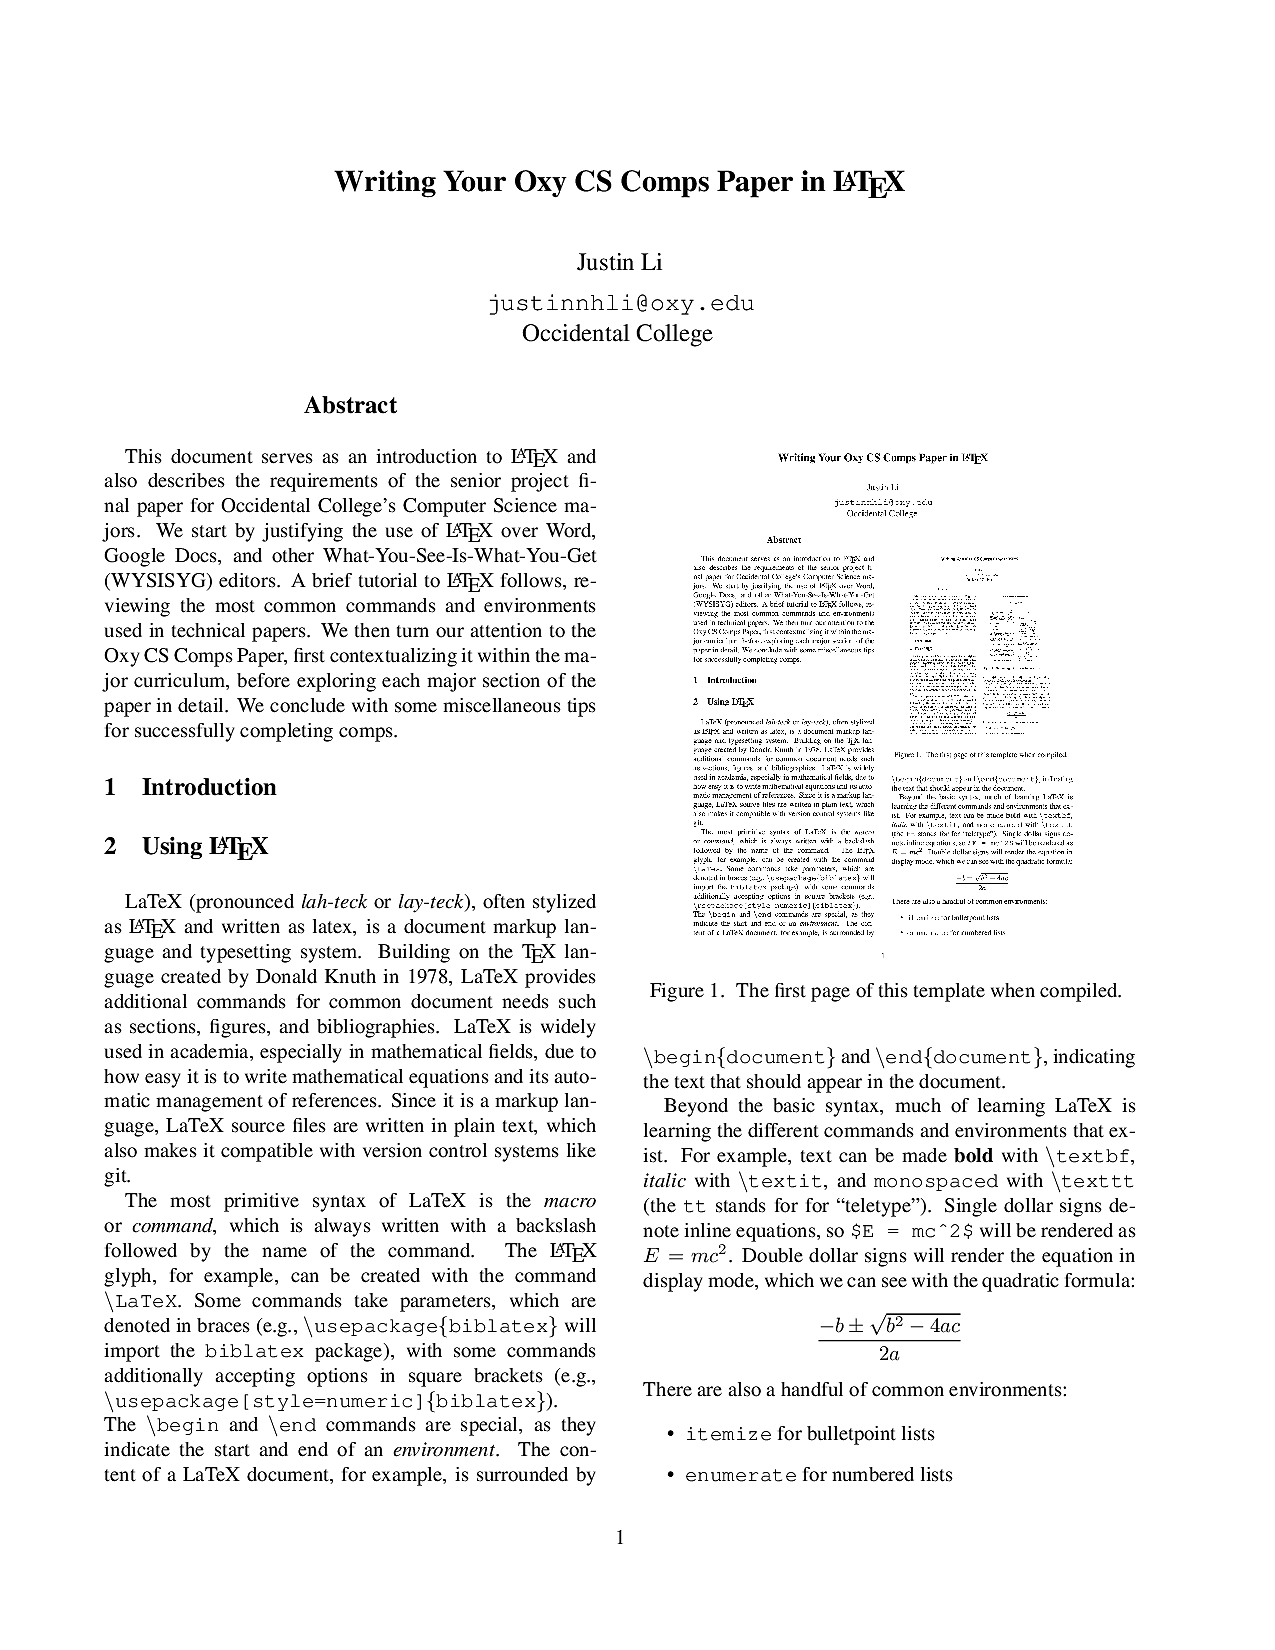
\includegraphics[width=.95\linewidth]{recursion.png}
    \caption{
        The current page of this paper, as an image.
    }
    \label{fig:first-page}
\end{figure}

Beyond the basic syntax, much of learning LaTeX is learning the different commands and environments that exist.
For example, text can be made \textbf{bold} with \texttt{\textbackslash textbf}, \textit{italic} with \texttt{\textbackslash textit}, and \texttt{monospaced} with \texttt{\textbackslash texttt} (the \texttt{tt} stands for for ``teletype'').
Single dollar signs denote inline equations, so \texttt{\$E = mc\textasciicircum 2\$} will be rendered as $E = mc^2$.
Double dollar signs will render the equation in display mode, which we can see with the quadratic formula:

$$\frac{{-b \pm \sqrt {b^2 - 4ac} }}{{2a}}$$

There are also a handful of common environments:

\begin{itemize}
    \item \texttt{itemize} for bulletpoint lists
    \item \texttt{enumerate} for numbered lists
    \item \texttt{figure} for figures (see Figure \ref{fig:first-page})
    \item \texttt{tabular} for tables
    \item \texttt{lstlisting} for code listings (see Listing \ref{lst:python-hello-world})
\end{itemize}

\begin{lstlisting}[
    language=Python,
    caption={Hello, World! in Python},
    label={lst:python-hello-world},
    float
]
def hello():
    print('hello, world!')
\end{lstlisting}

This covers the most frequently used commands, but as you might have already inferred, LaTeX is a vast and deep system, and can easily be overwhelming.
We recommended reading through the \citetitle{Overleaf2021LearnLaTeXIn} tutorial \cite{Overleaf2021LearnLaTeXIn} and using the \citetitle{WikiBook2022LaTeX} \cite{WikiBook2022LaTeX} as reference.
Beyond that, you should examine and play with the source of this document to gain working proficiency with LaTeX.

One final note on writing in LaTeX.
Since LaTeX is only a markup language, the source files must be compiled into a viewable form, most commonly into a PDF file.
The source of this document is made up of several files, each with its own purpose:
\begin{itemize}
    \item \texttt{template.tex} - The main LaTeX file containing the contents of the document.
    \item \texttt{oxycomps.sty} - A style file with settings for what the document should look like.
    \item \texttt{references.bib} - A list of bibliography items.
    \item Other files containing images, build instructions, etc.
\end{itemize}
Manual compilation of these files is somewhat esoteric, as it requires multiple uses of the \texttt{pdflatex} and \texttt{biblatex} commands.
Instead, it is much easier to use tools such as \texttt{pdflatex} or \texttt{latexmk} (in the terminal) or Overleaf (online) for compilation.
We have also provided a \texttt{Makefile} which will automatically update the document as necessary; the use of makefiles is beyond the scope of this document, but see \textcite{Lambert2021MakefileTutorial}.

\begin{comment}
No definition citations, unless the term itself is in dispute
Separate problem background from technical background
    Unclear if games and apps require much technical background
    The general structure of the framework might be better suited for the Architecture Overview section
        Eg. Flask uses decorators to associate functions with URLs
        Eg. Unity has scripts associated with objects and specific triggers, such as walking into an area, pressing a button, etc.
    Maybe a better name is "algorithmic background"?
        Should explore what does and doesn't count
            All ML counts
            App and game frameworks do not
        Framework vs. library?
            I like the idea of [inversion of control](https://martinfowler.com/bliki/InversionOfControl.html), but that may be too abstract for students to understand
        Heuristic: is understanding that system necessary to understand the results?
            Ie. How Flask or Unity works doesn't influence whether the app/game is useful/fun/engaging
            But how (say) linear regression works is highly relevant for why the results match/don't match the actual values
\end{comment}

\section{Sections of the Oxy CS Comps Paper}
\label{sec:paper}

\subsection{Introduction and Problem Context}

This section should motivate why the project is interesting both to you and to the computer science community or the general public.
You should also justify the difficult of the project.
As a rough guideline, your project should be either narrow but deep in a subfield of CS, or broadly reaching across subfields without being too shallow.
It should be comparable to the amount of work/content in an upper-level elective.

\subsection{Technical Background}

This section introduces the technical knowledge necessary to understand your project, including any terminology and algorithms.
You should assume that the reader is a CS undergraduate like yourself, but not necessarily familiar with AI/ML/HCI/apps/video games/etc. 

\subsection{Prior Work}

This section describes of related and/or existing work.
This could be scientific or scholarly, but may also be a survey of existing products/games.
The goal of this section is to put your project in the context of what has already been done.

\subsection{Methods}

This section describes what exactly you will be working on.
What are you building? How will it combine/incorporate ideas from the literature? Be specific about what you will be doing: talk about the specific algorithm you will implement/use, the specific dataset/platform/API, and what the outcome of your project will look like.
All of these decisions should be justified as well.

\subsection{Evaluation}

\subsubsection{Evaluation Metric}

This section describes how you will evaluate your project.
What will you be measuring, and how will you measure it?
You might think about what would result in an F, a C, or an A for comps.
Alternately, think about what are the minimal requirements for passing the class, what you might do if you had more time and resources, and what the best case scenario would be if everything went swimmingly.

\subsubsection{Results and Discussion}

\subsection{Ethical Considerations}

Are there any ethical concerns that might arise from your project?
You might think about whether your project perpetuates societal inequity (or could be used by others to do so), whether the data/platforms you are using is collected with informed consent and free of bias, and whether you might be subject to technological solutionism instead of working support/better the public infrastructure.
Include a discussion of how you plan to mitigate these issues in your project.

\subsection{Limitations, Future Work, and Conclusion}

\subsection{Timeline}

A timeline of major milestones, with specific items to be completed by specific dates/months.
Note that this timeline must start over the summer; otherwise you will unlikely have enough time to complete a project of the expected scope.
As part of the discussion around your timeline, talk about what you already know that would help you with the project, and what you expect to have to learn to be successful.
Include programming languages, technical concepts, as well as processes (e.g., user testing).

\subsection{Code Documentation}

This section will demonstrate that you have thought through the basics of how your code will work. You should include a diagram of the overall data flow of your program, including what the inputs and outputs of each component will be, and how they will be represented.

\subsection{Appendices}

\section{Tips and Advice}

\printbibliography 

\end{document}
